\documentclass[11pt]{article}

\usepackage[catalan]{babel}
\usepackage[utf8]{inputenc}
\usepackage{graphicx}
\usepackage{listings}
\usepackage{geometry}
\usepackage{fancyhdr}
\usepackage{pdflscape}
\usepackage{caption}

\geometry{a4paper}
\pagestyle{fancy}
\graphicspath{ {imatges/} }
\fancyhf{}
\lhead{\small{\leftmark}}
\rhead{\footnotesize{\rightmark}}
\cfoot{-\thepage-}
\renewcommand{\headrulewidth}{1.5pt}
\lstset{numbers=left, showstringspaces=false, captionpos=b}
\renewcommand{\lstlistlistingname}{Índex de fragments de codi}
\renewcommand{\lstlistingname}{Fragment de codi}


\begin{document}

\begin{titlepage}
\newcommand{\HRule}{\rule{\linewidth}{0.5mm}} % Defines a new command for the horizontal lines, change thickness here

\begin{center}

\textsc{\LARGE Universitat Politècnica de Catalunya (UPC)}\\[1.5cm]
\textsc{\Large Facultat d'Informàtica de Barcelona (FIB)}\\[0.5cm]
\textsc{\large Grau en Enginyeria Informàtica\\Especialitat en Tecnologies de la Informació}\\[1.5cm]

\HRule \\[0.4cm]
{\huge \bfseries Practical home multihoming with OpenWrt and Open Overlay Router}\\
\HRule \\[1.5cm]

{\Large \emph{Autor:}\\
Sergi Bartolomé Muñoz}\\[1cm]
{\large \emph{Director:}\\
Albert Cabellos Aparicio\\
(Departament d'Arquitectura de Computadors)\\[0.5cm]
\emph{Codirector:}\\
Alberto Rodríguez Natal\\
(Departament d'Arquitectura de Computadors)}

\vfill


\includegraphics[scale=0.3]{fib-upc}\\[1cm]

{\large 23 de juny de 2016}\\[3cm]

\end{center}
\end{titlepage}

\newpage
\setcounter{page}{0}					%BE CAREFUL
\thispagestyle{empty}
\mbox{}
\vfill

\newpage
\setcounter{page}{0}					%BE CAREFUL
\thispagestyle{empty}
\begin{abstract}
Anomenem \textit{multihoming} a la capacitat de connectar dues línies d'Internet a un mateix dispositiu. Aquesta característica és habitual en routers d'alta gamma, però la seva configuració en routers domèstics no és trivial.\\
\\
Aquest projecte pretén fer del \textit{multihoming} una funcionalitat accessible per a tothom qui vulgui gaudir-ne, automatitzant tota la configuració possible i requerint la mínima interacció per part de l'usuari. \\
\\
Per a fer-ho, s'utilitzarà l'arquitectura de xarxa \textit{LISP} mitjançant l'implementació \textit{OpenOverlayRouter} i sobre el sistema operatiu \textit{OpenWrt} \\
\\

\end{abstract}
\vfill
\renewcommand{\abstractname}{Resumen}
\begin{abstract}
Llamamos \textit{multihoming} a la capacidad de conectar dos líneas de Internet a un mismo dispositivo. Esta característica es habitual en routers de alta gama, pero su configuración en routers domésticos no es trivial.\\
\\
Este proyecto pretende hacer del \textit{multihoming} una funcionalidad accesible para todos los que quieran disfrutarla, automatizando toda la configuración posible y requiriendo la mínima interacción por parte del usuario. \\
\\
Para hacerlo, se usará la arquitectura de red \textit{LISP} mediante la implementación \textit{OpenOverlayRouter} i sobre el sistema operativo \textit{OpenWrt} \\
\\

\end{abstract}
\vfill

\renewcommand{\abstractname}{Abstract}
\begin{abstract}
Multihoming is the capabilty of connecting two Internet links to just one device. It is usual to find this feature in high-end routers, but its configuration in home devices is not trivial.\\
\\
This project aims to make \textit{multihoming} a feature available to everyone who wants to enjoy it, by automating all the possible configuration and by requiring as less user interaction as possible. \\
\\
To do it, we will be using the \textit{LISP} network arquitecture through the \textit{OpenOverlayRouter} implementation and over the \textit{OpenWrt} operating system\\
\\

\end{abstract}
\newpage
\setcounter{page}{0}					%BE CAREFUL
\thispagestyle{empty}
\mbox{}
\vfill

\newpage
\renewcommand{\thepage}{\roman{page}}
\setcounter{page}{1}
\tableofcontents
\lstlistoflistings
\listoffigures
\newpage
\renewcommand{\thepage}{\arabic{page}}
\setcounter{page}{1}					%BE CAREFUL
\section{Definició de l'abast i contextualització}
\subsection{Context}
\subsubsection{Introducció}
Aquest és un projecte de Treball de Fi de Grau (TFG) del Grau en Enginyeria Informàtica cursat a la Facultat d’Informàtica de Barcelona (FIB) de la Universitat Politècnica de Catalunya (UPC), i desenvolupat en el marc d’un projecte de col·laboració entre el Departament d’Arquitectura de Computadors (DAC) i Cisco Systems, anomenat Open Overlay Router (OOR).\\
\\
El projecte OOR es basa en l’arquitectura de xarxa Locator/ID Separation Protocol (LISP\cite{dino13}) implementada per Cisco Systems, la qual vol solucionar el problema d’escalabilitat d’Internet causat per la creixent quantitat de dispositius que s’hi connecten i la manca d’adreces per identificar-los. Per fer-ho, LISP separa semànticament els dos tipus de dispositius que s’hi connecten: els dispositius finals, que s’identifiquen mitjançant Endpoint Indentifiers (EIDs), i els dispositius que formen part de la capa d’enrutament, identificats per Routing Locators (RLOCs).\\
\\
La intenció d’OOR és oferir una implementació de codi obert de LISP compatible amb Linux, Android i OpenWrt, per tal que tothom qui vulgui pugui utilitzar aquest protocol en diferents sistemes operatius.\\
\\
OpenWrt, concretament, és una distribució de Linux per a dispositius incrustats (majoritàriament routers i mòdems), que ofereix unes opcions de configuració molt més extenses i personalitzables que els firmwares preestablerts habituals\cite{open16}. Una d’aquestes opcions és, com a exemple rellevant per aquest projecte, el multihoming.\\
\\
S’anomena multihoming a la capacitat d’un dispositiu de connectar-se a més d’una xarxa de computadors d’un o varis proveïdors d’Internet (ISP), sigui per augmentar la banda ampla disponible o la fiabilitat de la xarxa. Però per a poder-ho fer, el router en qüestió necessita un mínim de dos ports de Wide Area Network (WAN), i els routers domèstics habituals només en tenen un, limitant així la utilització d’aquesta funció a una gran part del mercat. Tot i això, mitjançant una personalització intensiva de la configuració d’OpenWrt, podem convertir un dels varis ports Local Area Network (LAN) d’un dispositiu domèstic en WAN mitjançant l’ús de Xarxes Locals Virtuals (VLANs). Malgrat això, aquesta configuració requereix amplis coneixements de xarxes de computadors i aconseguir-ho no està a l’abast de tothom.\\
\\
L’objectiu d’aquest projecte és crear una distribució basada en OpenWrt per un model de router domèstic concret, que integri OOR i que permeti multihoming, configurant la mínima quantitat de paràmetres possible. D’aquesta manera, qualsevol usuari que vulgui gaudir de les millores d’aquesta arquitectura ho podrà fer de la manera més còmode i senzilla.

\subsubsection{Actors implicats}
Mitjançant la creació d’aquesta distribució es facilita enormement l’adopció d’aquest protocol a qualsevol àmbit, i això afecta al rol de vàries persones.
\paragraph{Desenvolupador principal}
Serà l'única persona que desenvolupi el projecte, i s’encarregarà d’assolir totes les fites programades, documentar el projecte i finalment presentar-lo.
\paragraph{Equip d’OOR}
Quan el projecte estigui finalitzat, els dubtes i problemes derivats de la instal·lació i la posada en marxa d’OOR pels usuaris serà molt menor, ja que només caldrà indicar quin model de router han de comprar i proporcionar el binari instal·lador per el model concret. I també se’n beneficiaran en quan a base d’usuaris,  ja que la barrera de la dificultat en la seva preparació es veurà molt reduïda.
\paragraph{Cisco Systems}
Un altre beneficiat d’aquest projecte serà Cisco Systems, ja que permetrà que més routers utilitzin LISP, incrementant així el seu mercat i la seva competitivitat davant altres protocols similars.
\paragraph{Usuari final}
Degut a la fàcil instal·lació i la mínima configuració dels elements necessaris per utilitzar OOR, l’usuari final que vulgui fer-ne ús només haurà de seguir un petit manual en comptes d’haver d’invertir hores en preparar-ho, així que també se’n veuran beneficiats.
\newpage
\subsection{Estat de l'art}
\subsubsection{Multihoming}
El multihoming, com ja s’ha explicat a l’apartat anterior, permet que un sol router pugui connectar-se a més d’una línia WAN, siguin o no del mateix proveïdor. Aquesta capacitat ens aporta certs avantatges respecte a l'única connexió habitual:
\begin{itemize}
\item Més fiabilitat: si una de les línies de l’ISP falla, tenim més opcions per tal de no perdre els paquests que enviem o rebem.
\item Més rendiment: depenent de la destinació, la ruta d’algun ISP pot ser més ràpida que la dels altres. D’aquesta manera tenim més opcions on escollir. 
\end{itemize}
L’esquema típic d’una estructura de xarxa usant multihoming seria la següent, on un sol dispositiu té connectivitat a més d’un ISP.\\
\\
\begin{figure}[h]
	\centering
	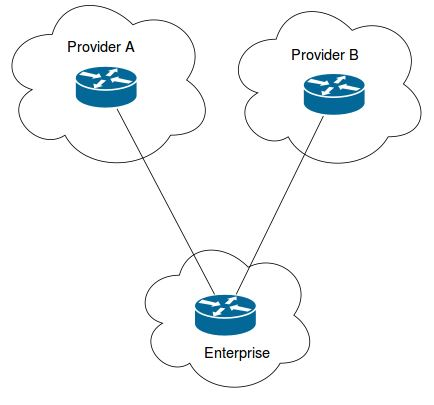
\includegraphics{multihoming}
	\caption{Estructura de xarxa usant multihoming}
\end{figure}
\\
En vista d'aquests avantatges, cada vegada més empreses, i fins i tot usuaris domèstics, consideren l'ús del multihoming com una opció factible, i cada vegada trobem més demanda d'aquest servei.

\subsubsection{LISP i OOR}
Per a permetre l’ús del multihoming s’ha escollit fer-ho mitjançant el projecte OOR, que a la vegada està basat en l’arquitectura de xarxa LISP.
LISP és un model de xarxa impulsat per l’IETF (Internet Engineering Task Force), la comunitat internacional de desenvolupadors l’objectiu de la qual és millorar la qualitat d’Internet. \\
\\
Les xarxes de computadors actuals utilitzen l’adreça IP per indicar la identitat del dispositiu, així com la manera com està connectat a la xarxa. Això provoca que el nombre d’adreces IP disponibles sigui molt baix, degut al creixement dels dispositius que utilitzen Internet (en part causat pel multihoming i l’èxit de l’Internet de les Coses (IoT), i LISP pretén solucionar el problema separant en dos espais de noms el “qui” i el “com” d’aquestes adreces IP, utilitzant un sistema de “mapping” per  relacionar les dues parts.\\
\\
L’estructura habitual d’un entorn de xarxa LISP és el mostrat a continuació:\\
\\
\begin{figure}[h]
	\centering
	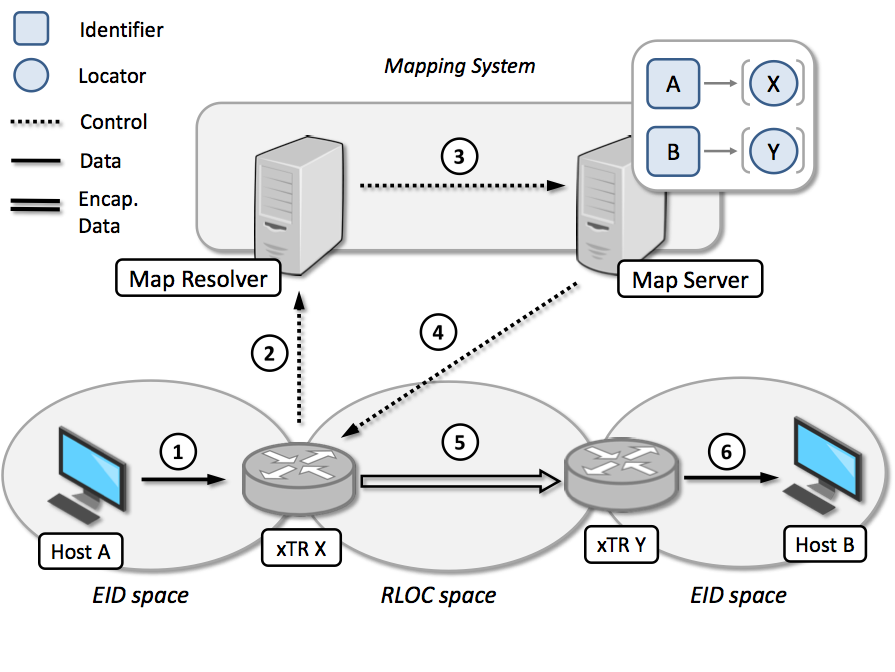
\includegraphics[width=14cm]{lisp}
	\caption{Entorn de xarxa LISP}
\end{figure}
\\
La xarxa on es troben els endhosts s’anomena EID Space i està vinculada a un xTR (un router compatible amb LISP). Aquests només es poden comunicar amb altres endhosts. Si formen part de diferents EID Spaces, l'xTR haurà d'atravessar la xarxa interna de LISP, consultant al Mapping System l'ubicació d'aquest EID Space (anomenada RLOC)\cite{alberto15}.
LISP es troba en un desenvolupament continu, optimitzant diferents paràmetres de l’arquitectura per a ser aplicats a resoldre varis problemes actuals\cite{freitas15},\cite{cisco15}.\\
\\
El seu objectiu és millorar tota l’estructura interna d’Internet i, per tant, és una arquitectura molt ambiciosa i es troba molt avançada tecnològicament respecte a la implementada actualment. \\
\\
Cisco Systems és un dels grans impulsors d’aquesta arquitectura, i l’ha implementat per a ser utilitzada sobre el sistema operatiu dels seus routers (IOS).\\
\\
OOR és l’opció de software lliure que treballa per oferir LISP a dispositius que utilitzin altres sistemes operatius, com ara Linux, Android i OpenWrt. El projecte va ser anunciat al 2011 per Cisco Systems i, tot i que va començar sent una implementació de mobilitat per LISP\cite{albert09}, la seva aportació ha augmentat dràsticament: ha passat a implementar tots els elements que formen l’arquitectura i hi està integrant tecnologies actuals com ara Open DayLight (ODL)\cite{alberts15}, oferint funcionalitat completa a totes les plataformes esmenades.

\subsubsection{OpenWrt}
Actualment, l’opció de software lliure més utilitzada, més extesa i amb la comunitat més activa en quant a sistemes operatius per a routers és OpenWrt. \\
\\
Nascuda al 2004, aquesta alternativa ofereix un sistema de fitxers totalment modificable, una interfície per a modificar-los i un gestor de paquets que permeten més accés i llibertat que el sistema tancat i poc personalitzable proporcionat pels fabricants d’aquest tipus de hardware.\\
\\
Per a dur a terme el projecte s’utilitzarà l’última versió estable d’aquell moment, en aquest cas la 15.05 Chaos Calmer, publicada el setembre de 2015.
\subsection{Abast del projecte}
\subsubsection{Objectius}
Com ja s’ha explicat, el projecte pretén facilitar el màxim possible la instal·lació i la posada en marxa de OOR. Per fer-ho, es seguiran els següents passos principals:
\begin{itemize}
\item Es buscarà un model de router relativament nou on centrar la distribució, que sigui compatible amb la última versió d’OpenWrt, que no tingui mòdem intern (ja que no compliria cap funció) i que permeti crear i gestionar VLANs.
\item Es cercarà la manera d’integrar tota la configuració de multihoming i d’OOR adequada dins d’un sol binari per facilitar al màxim la instal·lació a l’usuari final.
\item Es modificarà la interfície gràfica que proporciona OpenWrt perquè reflexi també els paràmetres d’OOR personalitzables.
\end{itemize}
\subsubsection{Possibles obstacles i solucions}
Durant el projecte poden sorgir certes complicacions i dificultats que afectin al seu desenvolupament i modifiquin la seva planificació temporal.
\begin{itemize}
\item La manca de disponibilitat del router escollit pot provocar un retard en el  desenvolupament. Solució: començar a fer proves amb un altre router compatible.
\item Errors de hardware al router on es treballarà. Solució: aconseguir més d’una unitat, si és possible, per si una falla.
\item Errors amb l’ordinador on es treballarà i possible pèrdua d’informació. Solució: el codi també s’emmagatzemarà en un gestor de versions.
\end{itemize}
\subsection{Metodologia}
\subsubsection{Mètode de treball}
S’utilitzarà la metodologia àgil Scrum, que ens permetrà gestionar el projecte de manera més amena i motivadora que amb un mètode més tradicional, ja que és adaptable a canvis i imprevistos i millora substancialment la productivitat. Tindrem reunions setmanals amb la resta de l’equip d’OOR.
\subsubsection{Eines de seguiment}
Quan es comenci a generar codi, aquest es gestionarà a través de Github, per així obtenir un control de versions i poder gestionar les modificacions i els canvis de la millor manera. A més, també permet treballar en local i en remot de manera fàcil i ràpida, tenint sincronitzat el repositori en tot moment a cada dispositiu des d’on es treballi.
També es seguirà un diagrama de Gantt per veure com avancen les tasques segons la planificació inicial.
\subsubsection{Validació}
Tota la feina es desenvoluparà en una sala amb gran part de l’equip d’OOR, per tant, qualsevol dubte al respecte podrà ser resolt de manera més o menys immediata, i les reunions setmanals serviran per validar la feina feta durant la setmana i discutir quin és el següent pas a seguir.


\section{Planificació temporal}
\subsection{Descripció de les tasques}
\subsubsection{Gestió del projecte}
La facultat requereix que, quan s’elabora un Treball de Fi de Grau (TFG), també es dugui a terme una assignatura addicional,  anomenada Gestió de Projectes (GEP). El seu objectiu és ajudar a encaminar el projecte i començar a documentar-lo des del principi, per tal que la memòria sigui complerta i la seva defensa posterior es realitzi correctament. A continuació es detallen els set lliurables a entregar, juntament amb les hores estimades per realitzar cada tasca.
\begin{enumerate}
\item Definició de l’abast i contextualització (7.1 hores)
\item Planificació temporal (4.6 hores)
\item Gestió econòmica i sostenibilitat (6.1 hores)
\item Presentació preliminar (3.6 hores)
\item Plec de condicions (7.6 hores)
\item Document final (12.1 hores)
\item Presentació final (11.1 hores)
\end{enumerate}
Sumant les hores indicades i les d’estudi de la matèria pertinents per cada lliurable, s’estima que la duració total serà de 75.2 hores.
Per dur-ho a terme s’utilitzarà un ordinador portàtil, Google Drive (per editar els lliurables des de qualsevol altre ordinador si fos necessari), un mòbil amb càmera (per editar el vídeo de la presentació preliminar), Dropbox (per compartir el vídeo de la presentació preliminar), Libre Office (per editar les rúbriques a entregar amb cada lliurable), Foxit Reader (per visualitzar els PDFs amb les rúbriques), Atenea (on entregar els lliurables), i el Racó de la FIB (on entregar el document final).
\subsubsection{Cerca del model de router}
El primer pas d’aquest projecte és escollir un router on centrar el seu desenvolupament, ja que el sistema OpenWrt depèn totalment del hardware d’aquest. Es durà a terme analitzant la llista de dispositius compatibles amb el sistema i haurà de complir amb els requisits que es detallen a continuació. El temps estimat a dedicar a la seva cerca és de 60 hores, i es necessitarà un ordinador proporcionat pel DAC, accés a Internet i Google Drive per llistar els models canditats abans de l’elecció.
\paragraph{Compatibilitat amb l'última versió d’OpenWrt}
Ja que el projecte està orientat a perdurar el màxim possible, el router haurà de ser compatible amb la versió més nova del sistema, per tal d'evitar actualitzacions del sistema a curt plaç.
\paragraph{Disponibilitat internacional}
El model escollit ha d’estar a la venta actual i internacionalment, ja que tothom ha de poder comprar-lo des d’arreu del món. Per tant, s’evitaran marques de producció només nacional o routers que ja no estiguin actualment en fabricació i distribució.
\paragraph{Compatibilitat amb VLANs}
El projecte necessita que el hardware amb el que es treballarà pugui crear i gestionar xarxes virtuals, i així poder configurar el multihoming definit a l'apartat anterior.
\paragraph{Especificacions adequades}
Si el router és dels últims del mercat i les seves característiques a nivell de hardware són prou altes, no caldrà renovar-lo ni a curt ni a mig plaç, ja que les característiques que ofereixin els nous models estaran igualades a les seves.
\subsubsection{Familiarització amb OpenWrt}
Al ser una distribució que no s’utilitza durant la carrera, s’hauran de dedicar vàries hores a familiaritzar-se amb el sistema i els seus dos mètodes d’interacció: UCI i LuCI. S’hi dedicaran aproximadament 60 hores en total, i serà necessari l’ordinador del DAC esmenat anteriorment, un mínim de tres targetes de xarxa connectades a ell, un mínim de tres cables de xarxa d’un metre, el model de router escollit i accés a Internet.
\subsubsection{Familiarització amb LISP i OOR}
L’arquitectura LISP i el projecte OOR que l’utilitza són nous i tampoc es veuen a cap assignatura del grau, per tant, caldrà també una familiarització amb ells i amb els seus fitxers de configuració (tant a Linux com a OpenWrt). Es pereveu dedicar-hi unes 60 hores. Per a fer-ho, caldrà l’ordinador del DAC amb les targetes de xarxa anteriors, cables de xarxa, el router escollit, vàries màquines virtuals i accés a Internet
\subsubsection{Configuració del multihoming}
El següent pas serà configurar un dels ports LAN del router, aïllat de la resta per una VLAN, com a port WAN. Això requerirà una estructura de xarxa OOR funcionant (amb vàries màquines virtuals implicades i ben configurades) i una configuració del router OpenWrt  correcta, així que necessitarà que totes les tasques anteriors hagin acabat. S’hi dedicaran 70 hores. En quant a requeriments físics, caldrà l’ordinador del DAC amb les seves targetes, cables de xarxa, dues línies WAN amb una adreça pública pròpia (S’usaran IPs de la UPC), el router i màquines virtuals.
\subsubsection{Automatització del multihoming}
La base del projecte és facilitar al màxim la configuració d’OOR i el multihoming a l’usuari final, per tant que aquest s’hagi de limitar a seguir el mínim de passos possible quan compri el router indicat. Per tant es buscarà la manera d’automatitzar tot el procés realitzat anteriorment, mitjançant scripts o amb la configuració prèvia d’arxius de OpenWrt OOR, i empaquetar-ho tot en una distribució independent. El temps estimat per a aquesta recerca i implementació serà de 70 hores, i es necessitarà també l’ordinador del DAC amb les seves targetes de xarxa, els cables de xarxa, les dues línies WAN amb adreça pública pròpia, el router i màquines virtuals.
\subsubsection{Adaptació de la interfície}
Al haver afegit multihoming i OOR integrats directament al sistema, s’haurà de modificar la interfície de configuració que usarà l’usuari final. Aquesta haurà de comptar amb paràmetres per configurar els detalls esmenats anteriorment i facilitar la seva modificació. S’hi dedicaran 60 hores i es requerirà l’ordinador del DAC amb les seves targetes de xarxa, cables de xarxa, dues línies WAN amb adreça pública pròpia, el router i màquines virtuals.
\subsubsection{Documentació i preparació de la defensa}
Finalment el projecte s’ha de documentar i defensar davant d’un tribunal de professors i doctors de la facultat. La redacció del document i la preparació de la defensa durarà unes 50 hores, i s’utilitzarà un ordinador portàtil o el proporcionat pel DAC, un editor de text compatible amb el llenguatge LaTeX, i un conversor de documents a PDF.

\subsection{Estimació del temps i seqüència de tasques}
\subsubsection{Temps estimat per tasca}
\begin{center}
	\begin{tabular}{| l | l |}
		\hline
		Tasca & Hores estimades \\ \hline
		Gestió del projecte & 75.2 \\ \hline
		Cerca del model de router & 60 \\ \hline
		Familiarització amb OpenWrt & 60 \\ \hline
		Familiarització amb LISP i OOR & 60 \\ \hline
		Configuració del multihoming & 70 \\ \hline
		Automatització del multihoming & 70 \\ \hline
		Adaptació de la interfície & 60 \\ \hline
		Documentació i preparació de la defensa & 60 \\ \hline
		Total & 515 \\ \hline
		\hline
	\end{tabular}
\end{center}

\subsubsection{Seqüència de les tasques i dependències}
\begin{center}
	\begin{tabular}{| l | l |}
		\hline
		Tasca & Tasca predecessora \\ \hline
		Gestió del projecte & - \\ \hline
		Cerca del model de router & - \\ \hline
		Familiarització amb OpenWrt & - \\ \hline
		Familiarització amb LISP i OOR & Familiarització amb OpenWrt \\ \hline
		Configuració del multihoming & Familiarització amb LISP i OOR \\ \hline
		Automatització del multihoming & Configuració del multihoming \\ \hline
		Adaptació de la interfície & Automatització del multihoming \\ \hline
		Documentació i preparació de la defensa & Adaptació de la interfície \\ \hline
		\hline
	\end{tabular}
\end{center}
\newpage
	\subsubsection{Diagrama de Gantt}
	La planificació temporal ha estat la següent:\\
	\begin{figure}[h]
		\centering
		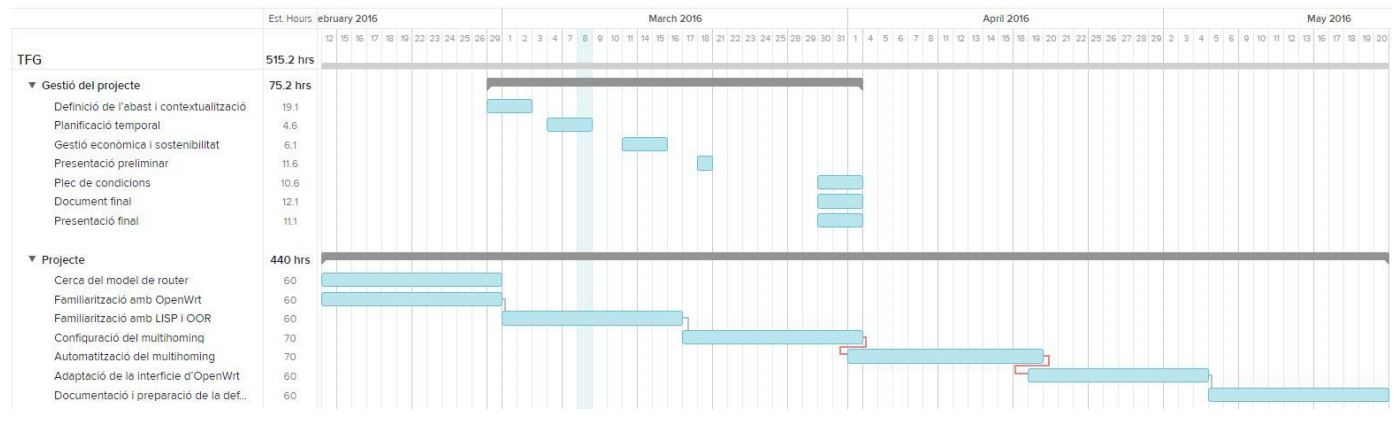
\includegraphics[width=14cm]{gantt1}
		\caption{Diagrama de Gantt del projecte}
	\end{figure}	

\subsection{Possibles complicacions i alternatives}
\subsubsection{Tardança en l’adquisició del router}
És possible que, degut a problemes de temps o poca disponibilitat econòmica del grup de recerca, la compra del router s’enradereixi. Tot i això, l’equip disposa de varis routers compatibles amb la última versió d’OpenWrt i es podria començar a fer proves amb aquests dispositius.
\subsubsection{Dificultats en la comprensió del sistema OpenWrt}
Al no haver utilitzat mai aquest sistema, pot ser que sorgeixin dubtes i dificultats a l’hora de compilar-lo o treballar-hi. Això pot retrassar lleugerament la data de finalització, ja que repercutiria a altres tasques, però la comunitat del sistema és molt activa i el seu fòrum presenta molta col·laboració a l’hora de resoldre dubtes i incompatibilitats.
\subsubsection{Dificultats en la comprensió de LISP i OOR}
Aquestes dues tecnologies també són molt novedoses, i caldrà molta investigació al respecte abans d’utilitzar-les. La seva complexitat en quant a arquitectura de xarxes també pot retrassar el projecte, però es treballarà en una sala amb gran part de l’equip de desenvolupament, els quals podran donar un cop de mà al desenvolupament i resoldre tots els dubtes que sorgeixin.
\subsubsection{Problemes amb les dues línies WAN}
Es pot donar el cas que alguna de les línies de Wide Area Network (WAN) que es necessiten per treballar amb multihoming fallin en algun moment concret, dificultant així la seva configuració i potser creant confusió quan el sistema falli. Tot i això, es pot treballar conceptualment i utilitzar màquines virtuals per fer una simulació totalment vàlida.

\subsection{Finalització del projecte}
Donat el diagrama de Gantt anterior, i comptant que la presentació final del projecte es durà a terme a finals de Juny, podem veure que el plaç per acabar el projecte és més que suficient. Si algun dels casos presentats anteriorment presentés un problema d’organització, hi ha un marge temporal més que acceptable per solucionar-lo i presentar el projecte a la data prevista.

\section{Gestió econòmica i sostenibilitat}
\subsection{Identificació dels costos}
\subsubsection{Pressupost}
Aquí es detalla el cost de cada element necessari per a dur a terme cada tasca, tal com s’indicaven en l’anterior apartat, indicant per a cada element el seu cost directe, indirecte, amortització, contingències i imprevistos. L’odinador de sobretaula és cedit pel repartament, de manera que el seu cost s’ha calculat segons preu de mercat seguint les seves característiques hardware, així com també el preu de les interfícies de xarxa i els cables corresponents.
\begin{center}
	\begin{tabular}{| l | l | l | l | l | l |}
		\hline
		Tasca & U. & Preu/u. & Vida útil & Amortització & Preu \\ \hline
		Costos directes & & & & & \\ \hline
		Gestió del projecte & & & & & \\ \hline
		Ordinador portàtil & 1 & 750 & 4 & (750/7936) * 75h = 7.08 & 7.08 \\ \hline
		Google Drive & 1 & - & - & 0 & 0 \\ \hline
		Càmera (Mòbil) & 1 & 300 & 4 & (300/7936) * 75h = 2.83 & 2.83 \\ \hline
		Dropbox & 1 & - & - & 0 & 0 \\ \hline
		Libre Office & 1 & - & - & 0 & 0 \\ \hline
		Foxit Reader & 1 & - & - & 0 & 0 \\ \hline
		Google Chrome & 1 & - & - & 0 & 0 \\ \hline
		Cerca del model de router & & & & & \\ \hline
		Ordinador de sobretaula & 1 & 500 & 4 & (500/7936) * 60h = 3.78 & 3.78 \\ \hline
		Google Chrome & 1 & - & - & 0 & 0 \\ \hline
		Google Drive & 1 & - & - & 0 & 0 \\ \hline
		Familiarització amb OpenWrt & & & & & \\ \hline
		Ordinador de sobretaula & 1 & 500 & 4 & (500/7936) * 60h = 3.78 & 3.78 \\ \hline
		Targeta de xarxa & 3 & 15 & 4 & (15/7936) * 60h = 0.113 & 0.113 \\ \hline
		Cable de xarxa & 3 & 2 & 4 & (2/7936) * 60h = 0.015 & 0.015 \\ \hline
		Router & 1 & 150 & 4 & (150/7936) * 60h = 1.13 & 1.13 \\ \hline
		Familiarització amb LISP i OOR & & & & & \\ \hline
		Ordinador de sobretaula & 1 & 500 & 4 & (500/7936) * 60h = 3.78 & 3.78 \\ \hline
		Targeta de xarxa & 3 & 15 & 4 & (15/7936) * 60h = 0.113 & 0.113 \\ \hline
		Cable de xarxa & 3 & 2 & 4 & (2/7936) * 60h = 0.015 & 0.015 \\ \hline
		Router & 1 & 150 & 4 & (150/7936) * 60h = 1.13 & 1.13 \\ \hline
		Configuració del multihoming & & & & & \\ \hline
		Ordinador de sobretaula & 1 & 500 & 4 & (500/7936) * 60h = 3.78 & 3.78 \\ \hline
		Targeta de xarxa & 3 & 15 & 4 & (15/7936) * 60h = 0.113 & 0.113 \\ \hline
		Cable de xarxa & 3 & 2 & 4 & (2/7936) * 60h = 0.015 & 0.015 \\ \hline
		Router & 1 & 150 & 4 & (150/7936) * 60h = 1.13 & 1.13 \\ \hline
		Línies WAN & 2 & - & - & 0 & 0 \\ \hline
		Automatització del multihoming & & & & & \\ \hline
		Ordinador de sobretaula & 1 & 500 & 4 & (500/7936) * 60h = 3.78 & 3.78 \\ \hline
		Targeta de xarxa & 3 & 15 & 4 & (15/7936) * 60h = 0.113 & 0.113 \\ \hline
		Cable de xarxa & 3 & 2 & 4 & (2/7936) * 60h = 0.015 & 0.015 \\ \hline
		Router & 1 & 150 & 4 & (150/7936) * 60h = 1.13 & 1.13 \\ \hline
		Línies WAN & 2 & - & - & 0 & 0 \\ \hline
		Adaptació de la interfície & & & & & \\ \hline
		Ordinador de sobretaula & 1 & 500 & 4 & (500/7936) * 60h = 3.78 & 3.78 \\ \hline
		Targeta de xarxa & 3 & 15 & 4 & (15/7936) * 60h = 0.113 & 0.113 \\ \hline
		Cable de xarxa & 3 & 2 & 4 & (2/7936) * 60h = 0.015 & 0.015 \\ \hline
		Router & 1 & 150 & 4 & (150/7936) * 60h = 1.13 & 1.13 \\ \hline
		Línies WAN & 2 & - & - & 0 & 0 \\ \hline
		\hline
	\end{tabular}
	\begin{tabular}{| l | l | l | l | l | l |}
		\hline
		Tasca & U. & Preu/u. & Vida útil & Amortització & Preu \\ \hline
		Documentació i defensa & & & & & \\ \hline
		Ordinador de sobretaula & 1 & 500 & 4 & (500/7936) * 60h = 3.78 & 3.78 \\ \hline
		Editor Vim & 1 & - & - & 0 & 0 \\ \hline
		PDFLaTeX & 1 & - & - & 0 & 0 \\ \hline
		Costos indirectes & & & & & \\ \hline
		Llum & 1 & 8 & - & & \\ \hline
		Quota d'Internet & 1 & 60 & - & & \\ \hline
		Total acumulat & & & & & 38.46 \\ \hline
		Contingència (5\%) & & & & & 1.92 \\ \hline
		Total (Abans del 21\% d'IVA) & & & & & 40.38 \\ \hline
		Total (Amb el 21\% d'IVA) & & & & & 48.85 \\ \hline
		\hline
	\end{tabular}
\end{center}
A la taula s’indiquen primer els costos directes (hardware, software i mà d’obra) a continuació els indirectes (llum, Internet), s’hi aplica la contingència (que s’estima d’un 5\% degut a que les complicacions, com ja es va indicar a l’anterior apartat, són molt fàcils de solventar) i per últim el 21\% de l’Impost del Valor Afegit (IVA). \\
\\
L’amortització s’ha calculat a partir dels dies hàbils de l’any 2016 (248), aplicats a 8h d’ús màxim diari i multiplicant cada element per les hores a usar-se a cada tasca.\\
\\
També s’ha calculat el cost dels recursos humans implicats en el projecte, calculant les hores de duració del projecte. Les hores que realitzarà l’autor són el total destinat al projecte, mentre que tant el director com el codirector realitzaran les hores relatives a les hores que l’autor serà al departament, que s’han calculat descomptant les dedicades a GEP i gran part de les dedicades a documentació i familiarització amb les tecnologies.
\begin{center}
	\begin{tabular}{| l | l | l | l |}
		\hline
		Rol & Hores de feina & Salari/hora & Cost estimat \\ \hline
		Autor del projecte & 515 & 8 & 4.120 \\ \hline
		Director del projecte & 280 & 20 & 5.600 \\ \hline
		Codirector del projecte & 280 & 20 & 5.600 \\ \hline
		Cost total & & & 15.320 \\ \hline
		\hline
	\end{tabular}
\end{center}

\subsubsection{Control de gestió}
S’utilitzaran les reunions setmanals per calcular si el temps i recursos invertits segueixen sent els correctes o si cal modificar-los, tot havent apuntat les hores setmanals empleades amb cada un dels elements esmenats anteriorment.

\subsection{Sostenibilitat}
Es puntuarà la sostenibilitat econòmica, social i mediambiental del projecte segons una sèrie de preguntes plantejades per l’equip de GEP.
\subsubsection{Dimensió econòmica}
\begin{itemize}
\item Existeix una avaluació de costos, tant de recursos materials com humans? Sí, s’ha avaluat el cost de tots els tipus de recurs.
\item El cost del projecte ho faria viable si hagués de ser competitiu? Sí, ja que l’inversió estalvia temps tant a gent de l’equip com als usuaris finals.
\item Està prevista o hi ha col·laboració amb algun altre projecte (acadèmic, empresa, associació, etc.? Sí, amb el departament ja anomenat.
\end{itemize}
\subsubsection{Dimensió social}
\begin{itemize}
\item Hi ha una necessitat real del teu producte / servei? Sí
\item Satisfer aquesta necessitat millora la qualitat de vida dels consumidors? Sí, ja que proporciona facilitat de posada en marxa i d’ús d’OOR.
\item El resultat del projecte, en què / com canviarà la vida de l'usuari? La facilitarà i simplificarà àmpliament si vol utilitzar multihoming i OOR.
\end{itemize}
\subsubsection{Dimensió ambiental}
\begin{itemize}
\item Quin consum tindran aquests recursos durant el desenvolupament del projecte i posteriorment durant la seva posada en marxa i vida útil? Baix, el mateix que tenia el router abans de ser configurat per OOR.
\item Quin consum i impacte ambiental tindria realitzar la mateixa activitat sense l'existència del teu TFG (estalvi de paper i altres materials i/o energia?) Estalvi d’energia quan es posa en marxa el dispositiu.
\item Durant el desenvolupament del teu producte es generarà algun tipus de contaminació? No de manera directe.
\item Amb la implantació del projecte s'augmenta o es disminueix la petjada ecològica? Es disminueix el consum energètic del grup d’OOR.
\end{itemize}
\subsubsection{Matriu de sostenibilitat}
A partir dels resultats anteriors, la matriu de sostenibilitat generada és la següent:
\begin{center}
	\begin{tabular}{| l | l | l |}
		\hline
		Econòmica & Social & Ambiental \\ \hline
		8/10 & 8/10 & 8/10\\ \hline
		\hline
	\end{tabular}
\end{center}

\section{Elecció del router}

\subsection{Cerca}
A l’hora d’escollir el router descrit anteriorment, s’ha consultat la pàgina de dispositius compatibles de la pàgina oficial d’OpenWrt\cite{opens16}. Es necessitava un router que funcionés amb l’última versió de al distribució, que acceptés la creació de xarxes virtuals i que encara es pogués trobar al mercat. Com la llista permet filtrar el resultats segons diferents característiques o funcionalitats dels dispositius, s’hi han aplicat els següents paràmetres:
\begin{itemize}
\item Device Type: Router
\item Availability: Available
\item Supported Current Rel: 15.05
\item VLAN: Yes
\item Modem: No
\end{itemize}
D’aquesta manera es redueix el nombre de possibles candidats a 63, que suposa un canvi substancial respecte als 1225 de la llista anterior.
Un cop filtrats, també s’han tingut en compte diversos factors que no podien ser aplicats a la llista:
\begin{itemize}
\item Que només hi hagués una versió del router al mercat, per evitar complicacions a l’hora de comprar-lo i per mantenir la compatibilitat.
\item Que la instal·lació d’OpenWrt mitjançant el firmware original del dispositiu fos molt senzilla, sense requerir una connexió via ssh o ftp.
\item Que el seu hardware fos de prestacions altes però no excessives per un router domèstic.
\item Que estigués a la venda internacionalment i disponible a les botigues online més importants (com Amazon).
\end{itemize}
Amb aquest últim filtre manual es van seleccionar alguns models i es van plantejar com a candidats vàlids a la reunió setmanal, juntament amb les seves característiques més destacables.
\newpage
\subsection{Candidats}
\subsubsection{Belkin F9K1115 v2}
\begin{itemize}
\item Any: 2014
\item Memòria Flash: 16MB
\item Memòria RAM: 128MB
\item Freqüència de CPU: 720MHz
\item Ports: 1 WAN, 4 LAN
\item Instal·lació d’OpenWrt: via firmware original
\end{itemize}

\subsubsection{Netgear R6100}
\begin{itemize}
\item Any: 2013
\item Memòria Flash: 128MB
\item Memòria RAM: 128MB
\item Freqüència de CPU: 560MHz
\item Ports: 1 WAN, 4 LAN
\item Instal·lació d’OpenWrt: via firmware original
\end{itemize}

\subsubsection{Linksys WRT1200AC}
\begin{itemize}
\item Any: 2015
\item Memòria Flash: 128MB
\item Memòria RAM: 250MB
\item Freqüència de CPU: 2x1300MHz
\item Ports: 1 WAN, 4 LAN
\item Instal·lació d’OpenWrt: via firmware original
\end{itemize}


Finalment, per la seva data de llançament i característiques de hardware, el router escollit per a desenvolupar-hi el projecte i crear-ne la distribució d’OpenWrt va ser el model Linksys WRT1200AC.\\
\\
Per a poder començar el desenvolupament del projecte el més aviat possible s’ha començat utilitzant com a base el model Netgear WNDR3800, ja que l’equip d’OOR comptava amb un exemplar d’aquest a l’oficina. La compra d’aquest router es va realitzar degut que era un model suficientment potent i molt utilitzat dins la comunitat d’OpenWrt i, ja que la seva base d’usuaris segueix sent molt activa i elevada, s’ha decidit proporcionar també una implementació del projecte per a aquest router, oferint així una opció més econòmicament assequible i més accessible per a qui ja disposi d’aquest model.\\
\\
Les característiques del Netgear WNDR3800 són les següents:
\begin{itemize}
\item Any: 2011
\item Memòria Flash: 16MB
\item Memòria RAM: 128MB
\item Ports: 1 WAN, 4 LAN
\item Instal·lació d’OpenWrt: via firmware original
\end{itemize}

\section{Entorn de treball i configuració}
Per tal de crear l’automatització de les configuracions, s’ha simulat una arquitectura de xarxa LISP amb OOR i multihoming on poder fer proves i verificar si les configuracions s’estan creant correctament. Per a fer-ho, s’ha utilitzat una màquina física, un router i tres màquines virtuals mitjançant Virtualbox.\\
\\
Aquesta ha estat la fase més costosa del projecte degut, en part, al desconeixement de l’arquitectura de xarxa LISP i dels fitxers d’OOR i també als errors trobats a l’hora de fer la configuració. Els errors s’han trobat tant a la configuració de les màquines virtuals com a la configuració del router i com a la configuració de xarxa de la màquina física, on el gestor de xarxa per defecte d’Ubuntu (NetworkManager) no guardava els canvis realitzats a les interfícies i no havia definit les rutes per defecte necessàries.

\subsection{Màquina física}
Actua com a equip principal del projecte, on s’hi ha cercat el model de router, creat i gestionat les màquines virtuals, configurat el router, creat els scripts d’automatització del sistema, creat la interfície de configuració i escrit part de la memòria del projecte.\\
\\
De cara a l’escenari OOR ha actuat com a endhost, amb adreça 192.168.1.128. La seva configuració de xarxa ha estat l’habitual, ja que els endhosts són independents de l’ús d’OOR.
També ha fet de pont de connexió entre les màquines virtuals. S’han connectat 4 cables de xarxa entre aquesta màquina i el router, que han servit pels següents propòsits:
\begin{itemize}
\item Connexió SSH per configurar i monitoritzar el router.
\item Connexió al router com a endhost de l’EID.
\item Simulació de la connexió de la màquina virtual que actua com a Map Server/Map Resolver.
\item Simulació de la connexió de la màquina virtual que actua com a Mobile Node.
\end{itemize}

\subsection{Màquina virtual: Map Server/Map Resolver}
S’hi ha fet una instal·lació minimalista de la versió 14.04 d’Ubuntu Server, ja que no es necessitava interfície gràfica, i s’ha fet un pont virtual a una de les interfícies de xarxa de la màquina física, com ja s’ha explicat anteriorment.\\
\\
En aquesta màquina s’hi han unit dos dels elements que formen part de l’entorn de xarxa LISP, ja que és un cas usual i, a més, facilitava el desplegament virtual d’aquesta. Així doncs, la seva funció és la de gestionar la base de dades que relaciona RLOCs amb EIDs i acceptar i respondre sol·licituds que facin referència a aquesta.\\
\\
La configuració d’OOR que s’ha emprat és la descrita a continuació:\\
\lstset{caption=Configuració d'OOR del Map Server/Map Resolver}
\begin{lstlisting}[frame=single]
################################################
#
# General configuration
#

debug                      = 0 
map-request-retries        = 2
log-file                   = /var/log/oor.log
 
operating-mode             = MS

################################################
#
# MS configuration
#

control-iface              = eth2

lisp-site {
    eid-prefix            	= 192.168.1.0/24
    key-type              	= 1
    key                   	= password
    iid				= 0
    accept-more-specifics	= true
}

lisp-site {
    eid-prefix            	= 192.168.4.1/32
    key-type              	= 1
    key                   	= password
    iid				= 0
    accept-more-specifics	= true
}
\end{lstlisting}

\subsection{Màquina virtual: Mobile Node}
S’hi ha fet una instal·lació i configuració idèntica a l’anterior. La primera intenció amb aquesta màquina era utilitzar-la com a segon xTR que anunciés un altre EID, i connectar-hi virtualment una tercera màquina virtual que actués com a endhost dins d’aquest. Finalment, però, es va decidir que actués com a Mobile Node (MN), que ens permet utilitzar-lo tant com a RLOC com a endhost dins del seu propi EID, estalviant així la creació i gestió d’una tercera màquina virtual.\\
\\
La configuració d’OOR que s’ha emprat és la descrita a continuació:\\
\lstset{caption=Configuració d'OOR del Mobile Node}
\begin{lstlisting}[frame=single]

################################################
#
# General configuration
#

debug                  = 0 
map-request-retries    = 2
log-file               = /var/log/oor.log
 
operating-mode         = MN

###############################################
#
# Tunnel Router general configuration
# Common for xTR, RTR & MN
#

encapsulation          = LISP

rloc-probing {
    rloc-probe-interval             = 30
    rloc-probe-retries              = 2
    rloc-probe-retries-interval     = 5
}

map-resolver        = {
	192.168.3.2
}

###############################################
#
# xTR & MN configuration
#

map-server {
        address        = 192.168.3.2
        key-type       = 1
        key            = password
        proxy-reply    = on
}

database-mapping {
    eid-prefix          = 192.168.4.1/32
    iid                 = 0
    rloc-address {
        address         = 192.168.3.3
        priority        = 0
        weight          = 0
    }
}

\end{lstlisting}

\subsection{Router}
Actua com a enrutador de tot el trànsit de l’escenari, i com a xTR dins de l’entorn d’OOR. Té configurades tres VLANs:
\begin{itemize}
\item WAN: assignada a un port físic del router, utilitzada com a port WAN per defecte.
\item WAN2: assignada a un port físic del router, utilitzada per simular la segona línia WAN.
\item LAN: reuneix la resta de ports del router, que són interfícies destinades a endhosts de la xarxa. Actualment, un dels ports destinats a aquesta VLAN és utilitzat per gestionar-lo via SSH i l’altre com a enllaç amb l’endhost.
\end{itemize}
La seva configuració d’OOR és la següent; la sintaxi és diferent als fitxers mostrats anteriorment, ja que OpenWrt utilitza un llenguatge d’scripting concret, UCI, que s’explica més endavant.\\
\lstset{language=sh, caption=Configuració d'OOR de l'xTR}
\begin{lstlisting}[frame=single]
config daemon
    option debug '2'
    option log_file '/tmp/oor.log'
    option map_request_retries '2'
    option operating_mode 'xTR'

config rloc-probing
    option rloc_probe_interval '0'
    option rloc_probe_retries '2'
    option rloc_probe_retries_interval '5'

config map-resolver
    list address '192.168.3.2'

config map-server
    option address '192.168.3.2'
    option key_type '1'
    option key 'password'
    option proxy_reply 'on'

config database-mapping
    option eid_prefix '192.168.1.0/24'
    option iid '0'
    option rloc_set 'external_ifs'

config rloc-set
    option name 'external_ifs'
    list rloc_name 'rloc_1'
    list rloc_name 'rloc_2'

config rloc-address
    option name 'rloc_1'
    option address '192.168.2.1'
    option priority '1'
    option weight '100'

config rloc-address
    option name 'rloc_2'
    option address '192.168.3.1'
    option priority '1'
    option weight '100'
\end{lstlisting}

\section{Automatització del multihoming}
Per tal de complir amb l’objectiu del projecte, s’ha cercat la manera òptima d’automatitzar la configuració dels fitxers de xarxa, OOR i firewall, de tal manera que l’interacció de l’usuari sigui mínima. Per a fer-ho, s’ha creat un script per a cada fitxer a modificar i finalment un que els agrupa i executa linealment. 
\subsection{UCI}
Els scripts s’han creat utilitzat la UCI command line, el llenguatge d’scripting dedicat d’OpenWrt, que ens permet llegir i modificar la configuració del sistema sense utilitzar parsing\cite{uci16}. Aquest es basa en l’anomenada Unified Configuration Interface (UCI), que pretén centralitzar tota la configuració d’OpenWrt en un conjunt de fitxers que s’ubiquen al mateix arbre de directoris i que segueixen la mateixa sintaxi. És un llenguatge poc flexible, ja que es tracta de l’edició de fitxers amb una estructura molt concreta i amb unes opcions limitades, però és també una manera molt còmode de canviar configuracions.
\subsection{Script principal}
Es limita a executar tot el conjunt d’scripts de configuració la primera vegada que OpenWrt s’executa al dispositiu. El seu contingut és el següent:\\
\lstset{language=sh, caption=Script principal d'automatització}
\begin{lstlisting}[frame=single]

# This file executes the configuration scripts to create a
# simple multihoming environment

# network.sh enables and configures multihoming on 
# the device
sh ./network.sh

# oor.sh configures OOR to work with a default configuration
sh ./oor.sh

# firewall.sh configures the firewall to allow multihoming 
# and OOR to work
sh ./firewall.sh
\end{lstlisting}

\subsection{Script d’inicialització}
S’ha d’assegurar que l’script anterior s’executi a l’inciar el sistema, però que només ho faci el primer cop. Per fer-ho, s’ha generat un script ubicat al directori /etc/init.d per tal que s’executi a l’inici i s’ha usat un fitxer buit per comprovar si aquest ja s’havia executat anteriorment: si el fitxer “firstboot.log” es troba al directori /scripts/ del sistema, significa que no és el primer cop que el sistema arrenca i, per tant, no cal generar la configuració. En el cas contrari, s’executaria l’automatització i es crearia el fitxer citat anteriorment.\\
\\
Aquest és el codi de l’script:\\
\lstset{language=sh, caption=Script per executar l'automatització només una vegada}
\begin{lstlisting}[frame=single]
#!/bin/sh
#sh /scripts/config.sh
FLAG="/scripts/firstboot.log"
if [ ! -f $FLAG ]; then
    sh /scripts/config.sh
    touch $FLAG
fi
\end{lstlisting}

\subsection{Network}
Edita el fitxer de configuració de la xarxa, ubicat a /etc/config/network. Crea les dues VPNs, les assigna als ports corresponents del router i guarda i recarrega la configuració per tal que els canvis s’apliquin.\\
\\
La configuració ha variat entre els dos models de router, tant per temes d'adreçament com per diferències entre el funcionament del switch dels dos dispositius.\\
\\
El seu contingut és el següent:\\
\lstset{caption=Script de configuració de la xarxa: WNDR3800}
\begin{lstlisting}[frame=single]

# This script edits the default network configuration from 
# OpenWrt and enables the use of multihoming in the device.
# To do so, it creates a VLAN that will be used as a WAN 
# interface, and then links it to a switch port.

# This sets a new VLAN that will act as a second WAN interface
uci set network.lan2='interface'
uci set network.lan2.ifname='eth0.2'
uci set network.lan2.proto='dhcp'
uci set network.lan2.metric='200'

# This lets the LAN interface act as a VLAN
uci set network.lan.ifname='eth0.1'

# We set a diffreent metric for the WAN interface
uci set network.wan.metric='100'

# This enables VLANs in the internal switch
uci add network switch
uci set network.@switch[-1].name='switch0'
uci set network.@switch[-1].reset='1'
uci set network.@switch[-1].enable_vlan='1'

# Here we assign the ports that will act as the LAN interfaces
uci set network.lans='switch_vlan'
uci set network.lans.device='switch0'
uci set network.lans.vlan='1'
uci set network.lans.ports='0 1 2 5t'

# Then we assign the VLAN we created to a fisical port
uci set network.wan2='switch_vlan'
uci set network.wan2.device='switch0'
uci set network.wan2.vlan='2'
uci set network.wan2.ports='3 5t'

uci commit network

# And finally we must reload the network configuration
/etc/init.d/network reload
\end{lstlisting}

\lstset{caption=Script de configuració de la xarxa: WRT1200AC}
\begin{lstlisting}[frame=single]
# This script edits the default network configuration from 
# OpenWrt and enables the use of multihoming in the device.
# To do so, it creates a VLAN that will be used as a WAN 
# interface, and then links it to a switch port.

# This sets a new VLAN that will act as a second WAN interface
uci set network.lan2='interface'
uci set network.lan2.ifname='eth1.3'
uci set network.lan2.proto='dhcp'
uci set network.lan2.metric='200'

# This lets the LAN interface act as a VLAN
uci set network.lan.ifname='eth1.1'

# We set a diffreent metric for the WAN interface
uci set network.wan.metric='100'

# This enables VLANs in the internal switch
uci add network switch
uci set network.@switch[-1].name='switch0'
uci set network.@switch[-1].reset='1'
uci set network.@switch[-1].enable_vlan='1'

# Here we assign the ports that will act as the LAN interfaces
uci set network.lans='switch_vlan'
uci set network.lans.device='switch0'
uci set network.lans.vlan='1'
uci set network.lans.ports='0 1 2 6t'

# We add the default VLAN configuration for the WAN port
uci set network.wan='switch_vlan'
uci set network.wan2.device='switch0'
uci set network.wan2.vlan='2'
uci set network.wan2.ports='4 5'

# Then we assign the VLAN we created to a fisical port
uci set network.wan2='switch_vlan'
uci set network.wan2.device='switch0'
uci set network.wan2.vlan='3'
uci set network.wan2.ports='3 6t'

uci commit network

# And finally we must reload the network configuration
/etc/init.d/network reload
\end{lstlisting}

\subsection{OOR}
Edita el fitxer de configuracó d’OOR, ubicat a /etc/config/oor. Assigna al router la funció d’xTR, assigna les dues interfícies que s’anunciaran com a RLOC i guarda i recarrega la configuració per tal que els canvis s’apliquin.\\
\\
També varia segons el model de router, ja que els noms de les interfícies utilitzades no són compartits.\\
\\
El seu contingut és el següent:\\
\lstset{caption=Script de configuració d'OOR: WNDR3800}
\begin{lstlisting}[frame=single]

# This script edits the default configuration file for OOOR
# to create a default multihoming environment

# TODO: Copy the example file to /etc/config/oor

# General configuration
uci set oor.@daemon[0].operating_mode='xTR'

# xTR configuration
uci set oor.@database-mapping[0].rloc_set='external_ifs'

#Miscellaneous configuration
uci set oor.@rloc-set[0].name='external_ifs'
uci set oor.@rloc-set[0].rloc_name='rloc_1'
uci add_list oor.@rloc-set[0].rloc_name='rloc_2'

# RLOC addresses
uci add oor rloc-iface
uci set oor.@rloc-iface[-1].name='rloc_1'
uci set oor.@rloc-iface[-1].interface='eth1'
uci set oor.@rloc-iface[-1].ip_version='4'
uci set oor.@rloc-iface[-1].priority='1'
uci set oor.@rloc-iface[-1].weight='100'

uci add oor rloc-iface
uci set oor.@rloc-iface[-1].name='rloc_2'
uci set oor.@rloc-iface[-1].interface='eth0.2'
uci set oor.@rloc-iface[-1].ip_version='4'
uci set oor.@rloc-iface[-1].priority='1'
uci set oor.@rloc-iface[-1].weight='100'

uci commit oor

/etc/init.d/oor reload
\end{lstlisting}
\newpage
\lstset{caption=Script de configuració d'OOR: WRT1200AC}
\begin{lstlisting}[frame=single]

# This script edits the default configuration file for OOOR
# to create a default multihoming environment

# TODO: Copy the example file to /etc/config/oor

# General configuration
uci set oor.@daemon[0].operating_mode='xTR'

# xTR configuration
uci set oor.@database-mapping[0].rloc_set='external_ifs'

#Miscellaneous configuration
uci set oor.@rloc-set[0].name='external_ifs'
uci set oor.@rloc-set[0].rloc_name='rloc_1'
uci add_list oor.@rloc-set[0].rloc_name='rloc_2'

# RLOC addresses
uci add oor rloc-iface
uci set oor.@rloc-iface[-1].name='rloc_1'
uci set oor.@rloc-iface[-1].interface='eth0'
uci set oor.@rloc-iface[-1].ip_version='4'
uci set oor.@rloc-iface[-1].priority='1'
uci set oor.@rloc-iface[-1].weight='100'

uci add oor rloc-iface
uci set oor.@rloc-iface[-1].name='rloc_2'
uci set oor.@rloc-iface[-1].interface='eth1.3'
uci set oor.@rloc-iface[-1].ip_version='4'
uci set oor.@rloc-iface[-1].priority='1'
uci set oor.@rloc-iface[-1].weight='100'

uci commit oor

/etc/init.d/oor reload
\end{lstlisting}


\subsection{Firewall}
Edita el fitxer de configuració del firewall, ubicat a /etc/config/firewall. Permet el forwarding entre les diferents interfícies (tants els RLOCs com l’EID) i també permet el tràfic entrant i sortint dels ports 4341 i 4342, necessaris pel funcionament d’OOR.\\
\\
En aquest cas, la configuració necessària per ambdós routers és la mateixa, de manera que només s'adjunta un dels codis.\\
\\
El seu contingut és el següent:\\
\lstset{caption=Script de configuració del firewall}
\begin{lstlisting}[frame=single]
# This script configures the firewall of OpenWrt to enable
# the use of OOR. We must allow traffic in ports 4341 
# and 4342, as well as forwarding them.

# First we will create a backup for the firewall file
cp /etc/config/firewall /etc/config/firewall_backup

# Then we will configure the required ports and interfaces 
# on the firewall configuration file
uci add firewall forwarding
uci set firewall.@forwarding[-1].src='wan'
uci set firewall.@forwarding[-1].dest='lan'

uci add firewall forwarding
uci set firewall.@forwarding[-1].src='lan'
uci set firewall.@forwarding[-1].dest='wan'

uci add firewall forwarding
uci set firewall.@forwarding[-1].src='wan'
uci set firewall.@forwarding[-1].dest='lan2'

uci add firewall forwarding
uci set firewall.@forwarding[-1].src='lan2'
uci set firewall.@forwarding[-1].dest='wan'

uci add firewall forwarding
uci set firewall.@forwarding[-1].src='lan'
uci set firewall.@forwarding[-1].dest='lan2'

uci add firewall forwarding
uci set firewall.@forwarding[-1].src='lan2'
uci set firewall.@forwarding[-1].dest='lan'

uci add firewall rule
uci set firewall.@rule[-1].name='Allow-4341-Input'
uci set firewall.@rule[-1].proto='udp'
uci set firewall.@rule[-1].src_port='4341:4342'
uci set firewall.@rule[-1].target='ACCEPT'

uci add firewall rule
uci set firewall.@rule[-1].name='Allow-4341-Output'
uci set firewall.@rule[-1].proto='udp'
uci set firewall.@rule[-1].dest_port='4341:4342'
uci set firewall.@rule[-1].target='ACCEPT'

uci add firewall rule
uci set firewall.@rule[-1].name='Allow-4341-Forwarding'
uci set firewall.@rule[-1].proto='udp'
uci set firewall.@rule[-1].src_port='4341:4342'
uci set firewall.@rule[-1].dest_port='4341:4342'
uci set firewall.@rule[-1].target='ACCEPT'

uci commit firewall

# Finally the firewall service must be restarted
/etc/init.d/firewall restart
\end{lstlisting}

\section{Creació de la interfície de configuració}
Encara que s’hagi automatitzat la configuració bàsica, l’usuari haurà de configurar manualment certs paràmetres d’OOR. Per tal que no hagi de lidiar amb scripts executats per línia de comandes ni editar fitxers manualment, s’ha utilitzat l’eina de configuració web oficial d’OpenWrt, LuCI.
\subsection{LuCI}
LuCI va sorgir degut a la falta d’una interfície de configuració simple, senzilla i fàcil d’ampliar per a dispositius incrustats. Utilitza el llenguatge de programació Lua i separa la interfície en diferents parts lògiques, com ara vistes i controladors, per tal de fer-la el més modular i pràctica possible.
A continuació es detallen els fitxers necessaris que s’han creat per implementar aquest mòdul.
\subsubsection{Model CBI}
Per a crear la vista del mòdul s’ha utilitzat el model CBI que proporciona LuCI, el qual crea una vista estil formulari amb els camps estipulats i directament modifica el fitxer corresponent amb les dades introduïdes per l’usuari, sense necessitat de crear una vista apart.\\
\\
Aquest és el codi que s'ha generat:\\
\lstset{caption=Model CBI de la interfície LuCI}
\begin{lstlisting}[frame=single]
m = Map("oor", "OOR Configuration")

s = m:section(TypedSection, "map-resolver",
		translate("Map Resolver"))
s.addremove = false
s.anonymous = true
s:option(Value, "address", "Address",
		"Encapsulated Map-Requests are sent to " ..
		"this map resolver (IPv4 or IPv6 or " ..
		"FQDN name)")

s = m:section(TypedSection, "map-server", "Map Server")
s.addremove = false
s.anonymous = true
s:option(Value, "address", "Address", "Register to this map" ..
		"server(IPv4 or IPv6 or FQDN name)")
s:option(Value, "key", "Key","Password to authenticate" ..
		"with the map-server")

s = m:section(TypedSection, "database-mapping",
		"Database Mapping")
s.addremove = false
s.anonymous = true
s:option(Value, "eid_prefix", "EID prefix", 
		"IPv4 or IPv6 network address of the OpenWrt" ..
		"LISP node / prefix length: x.x.x.x/x | " ..
		" y:y:y:y::y/y")
s:option(Value, "priority_v4",
		"IPv4 Priority","Priority of IPv4 locator " ..
		of	the interface for this EID. " ..
		"Locators with lower values are more " ..
		preferable. "A value of -1  means " ..
		"that IPv4 addres of that interface " ..
		"is not used [0-255]")
s:option(Value, "weight_v4", 
		"IPv4 Weight", "Weight of IPv4 " ..
		"locator of the	interface for this " ..
		"EID. When priorities are the same " ..
		"for multiple RLOCs, the Weight " ..
		"indicates how to balance unicast " ..
		"traffic between them [0-255]")
s:option(Value, "priority_v6",
		"IPv6 Priority","Priority of IPv6 " ..
		"locator of the interface for this EID." ..
		"Locators with lower values " ..
		"are more preferable. A value of " ..
		"-1  means that IPv6 address of " ..
		"that interface is not used [0-255]")
s:option(Value, "weight_v6", 
		"IPv6 Weight","Weight of IPv6 " ..
		"locator of the interface for this  EID." ..
		"When priorities are the same for " ..
		"multiple RLOCs, the Weight indicates " ..
		"how to balance unicast traffic between " ..
		"them [0-255]")

return m -- Returns the map
\end{lstlisting}

\subsubsection{Controlador}
És qui s’encarrega d’indicar on es troba el model, dir de quin tipus és i definir on i com apareix dins el menú principal de LuCI. El codi és el següent:\\
\lstset{caption=Controlador de la interfície LuCI}
\begin{lstlisting}[frame=single]
module("luci.controller.oor.oor", package.seeall)

function index()
    entry({"admin", "network", "interfaces"}, cbi("oor/oor"),
	"OOR Configuration", 30).dependent=false
end
\end{lstlisting}
\newpage
\subsubsection{Interfície web}
El resultat d’aquests fitxers és el mostrat a continuació. \\
\\
	\begin{figure}[h]
		\centering
		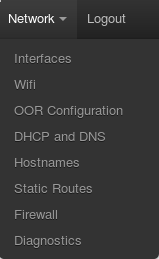
\includegraphics[scale=0.75]{luci1}
		\caption{Menú principal de LuCI, secció Network}
	\end{figure}	
	
Accedint al menú principal de LuCI, a la pestanya de Network, apareix l’opció de configurar OOR. Això ens porta al model CBI descrit anteriorment, on ens deixa modificar les opcions necessàries per a que OOR es pugui posar en marxa.\\

	\begin{figure}[h]
		\centering
		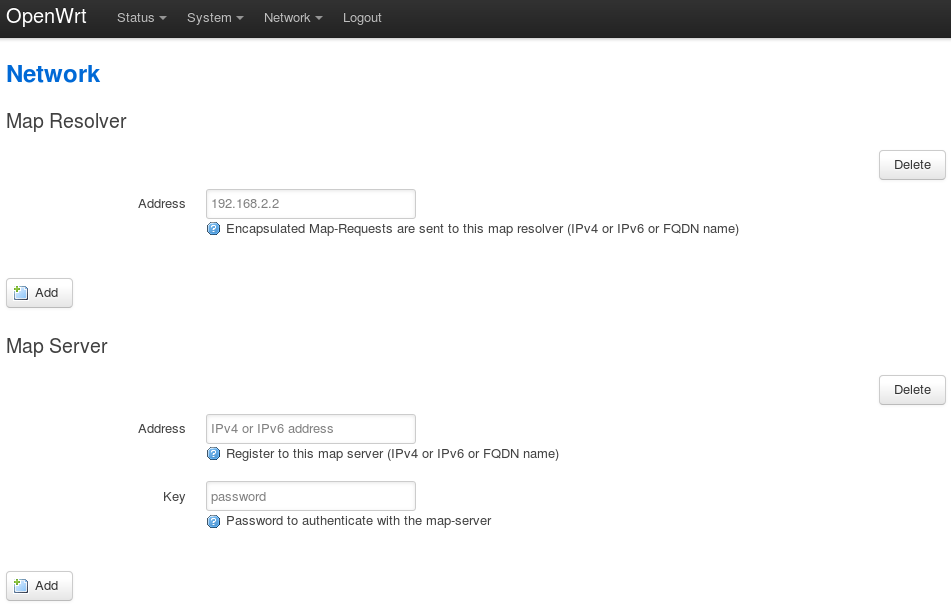
\includegraphics[width=15cm]{luci2}
		\caption{Pàgina de configuració d'OOR a LuCI}
	\end{figure}	

Com es pot observar, el mòdul ens demana les dades en un formulari, que a continuació modificarà automàticament el fitxer de configuració d’OOR. Es demanen només els paràmetres estrictament necessaris per tal que OOR pugui executar-se correctament i s'han exclòs les opcions més avançades per mantenir la facilitat d'ús de la interfície.
\newpage
\section{Generació de la imatge final}
Un cop preparada tota l’automatització del sistema, s’ha creat un fitxer binari d’instal·lació amb tota aquesta configuració inclosa. S’ha fet utilitzant l’OpenWrt Build System amb els següents paràmetres, apart dels activats per defecte:
\begin{itemize}
\item Target System: Marvell Armada 37x/38x/XP
\item Target Profile: Linksys WRT1200AC (Caiman)
\item Target Images: squashfs
\item LuCI: luci / lucisl
\item Network: SSH / oor
\end{itemize}

Per tal d’incloure els fitxers necessaris per l’automatització dins la imatge, s’ha creat el directori files/ a l’arrel d’OpenWrt i s’hi han inclòs els següents fitxers:
\begin{itemize}
\item files/scripts/config.sh
\item files/scripts/network.sh
\item files/scripts/oor.sh
\item files/scripts/firewall.sh
\item files/etc/init.d/config\_mh
\item files/usr/lib/lua/luci/controller/oor/oor.lua
\item files/usr/lib/lua/luci/model/cbi/oor/oor.lua
\end{itemize}
A continuació s’ha seguit la següent cadena de comandes dins una terminal: per compilar el sistema:
\begin{itemize}
\item cd openwrt/
\item ./scripts/feeds update -a
\item ./scripts/feeds install -a
\item make V=s
\end{itemize}
El resultat és una imatge de sistema compilada i llesta per ser carregada des del firmware oficial del router.
\newpage
\section{Manual d’usuari}
Finalment, es presenta una guia dels passos a seguir per configurar el sistema, en forma de petit manual i amb ajuda de captures de pantalla per tal que qualsevol usuari pugui seguir-lo fàcilment. En aquesta memòria es presenta una versió simplificada del manual.\\
\\
Primer s'accedeix a la direcció per defecte del router, 192.168.1.1, a través del navegador, on veurem la interfície web del firmware per defecte, amb aquest menú mostrat a l'esquerra.

\begin{figure}[h]
		\centering
		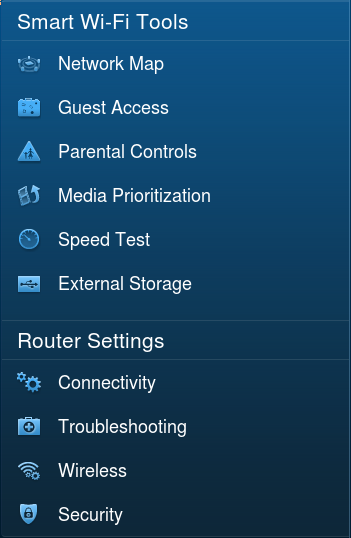
\includegraphics[scale=0.4]{man1}
		\caption{Manual de configuració: Connectivitat}
	\end{figure}
	
Des d'aquí clicarem l'opció Connectivity que ens mostrarà, entre d'altres, l'opció de carregar nosaltres mateixos una actualització del firmware. Ho utilitzarem doncs per instal·lar la nostra imatge d'OpenWrt.
\begin{figure}[h]
		\centering
		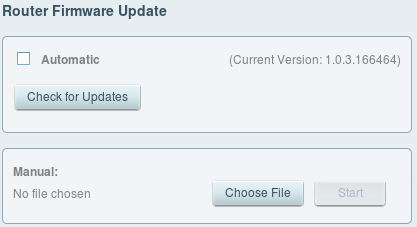
\includegraphics[scale=0.5]{man2}
		\caption{Manual de configuració: Càrrega}
	\end{figure}
\\
\\
	A continuació el dispositiu es reiniciarà i la pàgina es tornarà a carregar automàticament, aquesta vegada mostrant la pàgina principal de LuCI. Ens demanarà que assignem una contrasenya per accedir de manera segura al router i l'introduïrem.
\begin{figure}[h]
		\centering
		
\includegraphics[scale=0.5]{man3}
		\caption{Manual de configuració: Contrasenya}
	\end{figure}

Un cop acabat aquest pas, només quedarà connectar els cables de xarxa tal i com s'indica a la figura i configurar OOR utilitzant la interfície mostrada anteriorment.	
\begin{figure}[h]
		\centering
		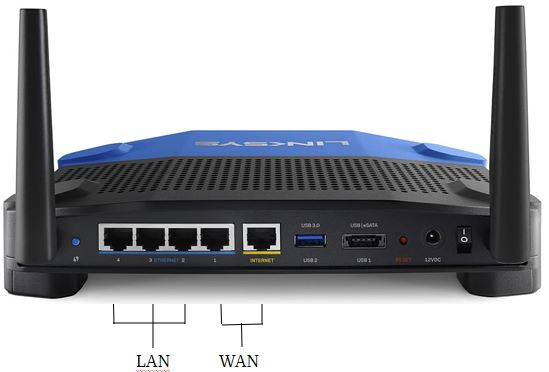
\includegraphics[scale=1]{linksys}
		\caption{Manual de configuració: Connexions de xarxa}
	\end{figure}
	
	
\section{Resultats}
A la data d’entrega de la memòria s’ha pogut configurar, automatitzar i executar correctament la funcionalitat de multihoming utilitzant OOR amb el model Netgear WNDR3800. S’ha capturat tràfic de xarxa sortint del router balançejat entre les dues interfícies WAN dirigit al Mobile Node, fet que verifica l’efectivitat de la configuració.\\
\\
Pel que fa al model Linksys WRT1200AC també s’hi ha configurat i automatitzat el multihoming, però encara s’hi estan analitzant detalls concrets del router que, al moment d’entrega d’aquesta memòria, no permeten l’execució totalment satisfactòria de la funcionalitat de multihoming en aquest dispositiu.

\section{Conclusions}
OpenWrt és una plataforma molt oberta i infinitament personalitzable, i això fa que per un usuari normal sigui un sistema complicat i costós de configurar, sobretot si es vol fer mitjançant línia de comandes o si s’hi volen aplicar mòduls complexos com ara OOR. Aquesta automatització facilita molt la posada en marxa del multihoming i d’OOR, requerint una interacció mínima per part de l’usuari.\\
\\
L'objectiu del projecte era precisament fer d'aquesta configuració una tasca trivial per part de l'usuari i es pot afirmar que s'ha complert amb l'objectiu. La primera part de la configuració es fa de manera totalment transparent i la part de configuració web s'ha pogut simplificar al màxim demanant només la introducció d'uns quants paràmetres.\\

\section{Feina futura}
La principal feina a fer és solucionar els detalls que no han permès la correcta execució del multihoming al model Linksys WRT1200AC.\\
\\
Mentre aquest projecte s'estava duent a terme, una part de la comunitat d'OpenWrt va crear un \textit{fork} del sistema operatiu degut a desavinences amb l'equip principal de desenvolupament. Al seu projecte l'han anomenat LEDE (Linux Embedded Development Environment), i sembla que també l'enfocaran a altres tipus de dispositius inscrustats i no només a routers i modems\cite{lede16}.\\
\\
Durant una reunió amb l'equip d'OOR es va proposar crear un binari d'instal·lació similar al ja generat, però utilitzant LEDE com a base. El binari s'ha compilat i preparat, però no s'ha pogut provar a cap dels dos routers utilitzats. La següent feina a dur a terme, per tant, seria comprovar que aquesta imatge també funciona i també configura la funció de multihoming correctament.


\begin{thebibliography}{9}

\bibitem{dino13}
  D. Farinacci, V. Fuller, D. Meyer, D. Lewis,
  \emph{The Locator/ID Separation Protocol (LISP)},
  Internet Engineering Task Force (IETF) RfC: 6830,
  2013.
\bibitem{open16}
  OpenWrt Community,
  \emph{About OpenWrt},
  https://wiki.openwrt.org/about/start.
  2016.
\bibitem{alberto15}
  A. Rodríguez, M. Portoles, V. Ermagan, D. Lewis, D. Farinacci, F. Maino,A. Cabellos,
  \emph{LISP: A southbound SDN protocol?},
  IEEE Communications Magazine 53 (7), 201-207,
  2015.
\bibitem{freitas15}
  S. Freitas, P. Bellagamba, N. Masterson,
  \emph{Preserving IP addresses during DC migration with LISP and ASR 1000},
  Cisco Systems White Paper,
  2015.
\bibitem{cisco15}
  Cisco Systems,
  \emph{Optimizing Ingress Routing with LISP across Multiple VXLAN/EVPN Sites.},
  Cisco Systems White Paper,
  2015.
\bibitem{albert09}
  Rodriguez-Natal, Alberto, Loránd Jakab, Marc Portolés, Vina Ermagan, Preethi Natarajan, Fabio Maino, David Meyer, and Albert Cabellos-Aparicio,
  \emph{LISP-MN: mobile networking through LISP.},
  Wireless personal communications 70, no. 1,
  2013.
\bibitem{alberts15}
  Open Overlay Router Community,
  \emph{What is OOR?.},
	https://github.com/OpenOverlayRouter/oor/wiki.
	2015.
\bibitem{opens16}
  OpenWrt Community,
  \emph{Table of Hardware.},
	https://wiki.openwrt.org/toh/start.
	2016.
\bibitem{uci16}
  OpenWrt Community,
  \emph{The UCI System.},
	https://wiki.openwrt.org/doc/uci.
	2016.
\bibitem{lede16}
  LEDE Community,
  \emph{About the LEDE Project.},
	https://www.lede-project.org/about.html.
	2016.
	
\end{thebibliography}

\end{document}